\documentclass[10pt,a4paper]{article}
\usepackage[margin=1.5cm]{geometry}
\usepackage[T1]{fontenc}
\usepackage{lmodern}
\usepackage{textcomp}
\usepackage{booktabs}
\usepackage{adjustbox}
\usepackage{amsmath}
\usepackage{enumitem}
\usepackage{listings}
\usepackage{xcolor}
\usepackage[hidelinks]{hyperref}
\usepackage{pgfplots}
\pgfplotsset{compat=1.18}
\definecolor{c1}{HTML}{2A78D6}
\definecolor{c2}{HTML}{EB6834}
\definecolor{c3}{HTML}{1BAF7A}
\definecolor{c4}{HTML}{EDA100}
\definecolor{c5}{HTML}{8F5BD6}

\usepackage{caption}
\captionsetup[lstlisting]{font=small,skip=2pt}
\lstdefinelanguage{Go}{
  morekeywords={break,case,chan,const,continue,default,defer,else,fallthrough,for,func,go,
    goto,if,import,interface,map,package,range,return,select,struct,switch,type,var,any},
  sensitive=true, morecomment=[l]{//}, morestring=[b]", morestring=[b]`}

\setlist{nosep,leftmargin=*}
\lstset{basicstyle=\ttfamily\small,columns=fullflexible,frame=single,framerule=0.3pt,
  rulecolor=\color{gray},breaklines=true,xleftmargin=2pt,xrightmargin=2pt,
  keywordstyle=\bfseries\color{c1!80!black},commentstyle=\itshape\color{black!55},
  stringstyle=\color{c2!80!black},showstringspaces=false}
\setlength{\parskip}{0.4em}
\setlength{\parindent}{0pt}
\setlength{\emergencystretch}{3em}

\title{Generic vs.\ non-generic Poseidon2 and Fiat--Shamir\\\large Benchmark report, \texttt{prover-ray/crypto/genericbench}}
\author{}
\date{28 October 2026}

\begin{document}
\maketitle
\vspace{-2em}

\section{Summary}

\begin{itemize}
  \item The fully generic Poseidon2 code is about \textbf{7--10$\times$ slower} than the
    non-generic baseline on KoalaBear and about \textbf{3$\times$ slower} on MamaBear.
    KoalaBear's gap is larger because its baseline uses gnark-crypto's AVX-512 assembly.
  \item The code the prover runs today (\texttt{current}: the generic hasher and transcript
    over gnark-crypto's compression) is \textbf{on par with the baseline} (within 2\%).
    Production is not affected.
  \item The root cause of the generic overhead is Go's implementation of generics: field
    operations are indirect calls that cannot be inlined, and they force local variables onto
    the heap. The generic permutation made 222--340 heap allocations per call.
  \item Branching to concrete KoalaBear code inside the permutation's hot loops removes all
    allocations from the permutation. With gnark-crypto's formulas replicated, it is about
    \textbf{3.5$\times$ faster} than the fully generic code, but still
    \textbf{2.6--2.9$\times$ slower} than baseline (2.2--2.6$\times$ for hashing and
    Fiat--Shamir).
  \item Where gnark-crypto's scalar code uses a cheaper formula, the generic code now uses
    the same one, so that the comparison measures genericity rather than different
    formulas. This applies to the internal matrix (Section~\ref{sec:replicate}). One
    MamaBear-specific trick is not replicated yet.
  \item Delegating the whole KoalaBear permutation to gnark-crypto's assembly
    (\texttt{generic-asm}) \textbf{matches the baseline} for the permutation itself.
    Batched \texttt{koalabear.Vector} operations inside the hot loops
    (\texttt{generic-vec}) are \textbf{about 20$\times$ slower} and are a dead end.
  \item The remaining gap comes from \textbf{2 heap allocations per compression} in the
    generic \texttt{Compress} function. Under parallel load (\texttt{CompressParallel},
    192 threads) they make the code about 16$\times$ slower than baseline, because of
    \textbf{garbage collection}: with the GC switched off the gap shrinks to 1.5$\times$.
    Removing these allocations is the next thing to fix.
\end{itemize}

\section{Setup}

\paragraph{Machine.} Intel Xeon Platinum 8488C, 192 cores, AVX-512 available (so the KoalaBear
baseline runs gnark-crypto's assembly path), Linux amd64, Go 1.27.1, gnark-crypto v0.22.0.
Nothing else ran on the machine during the benchmarks.

\paragraph{Implementations compared.} Each benchmark name ends in \texttt{impl=\dots}:
\begin{itemize}
  \item \texttt{baseline}: non-generic code. For KoalaBear, gnark-crypto's permutation and
    compression, and the pre-generic MD hasher and transcript (frozen in
    \texttt{legacy\_test.go}). For MamaBear, which never had a non-generic hasher,
    gnark-crypto's permutation under the generic hasher and transcript.
  \item \texttt{current} (KoalaBear only): what the prover runs today.
  \item \texttt{generic}: everything generic, permutation included. It appears under two
    column names, because the code changed between runs:
    \begin{itemize}
      \item \emph{fully generic} (Tables~\ref{tab:mid-kb} and \ref{tab:mid-mb}): before
        any branching;
      \item \emph{generic + hot-loop branches} (Tables~\ref{tab:kbb} and \ref{tab:paths}):
        the permutation's hot loops branch to concrete KoalaBear code
        (Section~\ref{sec:branch}).
    \end{itemize}
  \item \texttt{generic-vec}, \texttt{generic-asm} (KoalaBear only): the two alternative
    branches of Section~\ref{sec:paths}.
\end{itemize}

\paragraph{Runs.} Four runs, each preceded by \texttt{TestAgreement}, which checks that all
implementations produce bit-identical outputs. It passed every time.
\begin{center}\small
\begin{adjustbox}{max width=\linewidth}
\begin{tabular}{llll}
\toprule
Run & Code & Sizes & Samples \\ \midrule
1 (Tables~\ref{tab:mid-kb}, \ref{tab:mid-mb}) & \texttt{3ce6cc6e5}, fully generic & \texttt{full}, minus FS rounds=4096/update=16384 & $6\times500$\,ms \\
2 (Table~\ref{tab:kbb}, ``initial'') & \texttt{6b3d84ad3}, branches and the three paths & \texttt{medium}, KoalaBear only & $6\times200$\,ms \\
3 (Tables~\ref{tab:kbb}, \ref{tab:paths}) & run 2 + gnark-crypto diagonal replicated & \texttt{medium}, both fields & $6\times200$\,ms \\
4 (Table~\ref{tab:parallel}) & same code as run 3 & CompressParallel, KoalaBear, 1--192 threads & $6\times200$\,ms \\
\bottomrule
\end{tabular}
\end{adjustbox}
\end{center}
The single skipped FiatShamir case took about 40\,s per operation in the generic code and
dominated the runtime. Tables report the median of 6 samples. Unless noted otherwise, every
difference against the baseline is statistically significant according to \texttt{benchstat}
($p = 0.002$). The exceptions are \texttt{current} on MDHasher $n=2^{20}$ in run 1
($p=0.065$), on FiatShamir rounds=16/update=8 in run 3 ($p=0.065$) and on MDHasher $n=4096$
in run 3 ($p=0.026$). All are differences of under 2\%. Run 2 survives only as the medians
in \texttt{report/data/paths-run2-medians.csv}; its raw output was lost.

\section{Background: what is benchmarked}

All the benchmarks are built on the \textbf{Poseidon2 permutation}, the core of the Poseidon2
hash. It takes a fixed-size state of 16 or 24 field elements and scrambles it into another
state of the same size. It is reversible, hence ``permutation''. It runs 27 rounds (6 full,
21 partial), each made of three steps:
\begin{enumerate}
  \item \textbf{Add round keys}: add fixed constants derived from a seed.
  \item \textbf{S-box}: cube each element, $x \mapsto x^3$. This is the nonlinear step that
    gives the hash its security. Full rounds cube every element; partial rounds cube only the
    first.
  \item \textbf{Linear mixing}: multiply the state by a fixed matrix, so every element
    affects every other. Full rounds use the ``external'' matrix built from $4\times4$
    blocks (M4); partial rounds use the cheaper ``internal'' matrix $\mathbf{1}\mathbf{1}^T
    + D$.
\end{enumerate}
The other benchmark families are built on the permutation:
\begin{itemize}
  \item \textbf{Compress}: two 8-element blocks form a width-16 state, which is permuted;
    the second block is then added back (feed-forward). \textbf{CompressParallel} runs the
    same with one goroutine per hardware thread (192 threads on 96 cores).
  \item \textbf{MDHasher}: hashes $n$ elements, 8 at a time, with one compression per chunk.
  \item \textbf{FiatShamir}: a protocol-shaped transcript. Each round absorbs \texttt{upd}
    elements, samples a digest, samples query indices and derives a named challenge.
\end{itemize}
The permutation dominates every benchmark, so its speed carries through to all of them.

\section{Results 1: fully generic code}\label{sec:generic}

\begin{table}[htbp]\centering\small
\caption{KoalaBear, fully generic code (before any branching). Ratios are time relative to \texttt{baseline}.}\label{tab:mid-kb}
\begin{adjustbox}{max width=\linewidth}
\begin{tabular}{lrrrrr|rrr}
\toprule
Benchmark & baseline & fully generic & ratio & \texttt{current} & ratio & allocs \texttt{baseline} & allocs fully generic & allocs \texttt{current} \\ \midrule
Permutation (width=16) & 570\,ns & 5.18\,\textmu s & 9.09$\times$ & -- & -- & 0 & 222 & -- \\
Permutation (width=24) & 706\,ns & 7.43\,\textmu s & 10.5$\times$ & -- & -- & 0 & 298 & -- \\
Compress & 585\,ns & 5.22\,\textmu s & 8.91$\times$ & -- & -- & 0 & 224 & -- \\
CompressParallel & 4.31\,ns & 967\,ns & 224$\times$ & -- & -- & 0 & 224 & -- \\
MDHasher (n=8) & 733\,ns & 4.96\,\textmu s & 6.77$\times$ & 627\,ns & 0.86$\times$ & 5 & 225 & 1 \\
MDHasher (n=64) & 4.99\,\textmu s & 39.3\,\textmu s & 7.87$\times$ & 4.88\,\textmu s & 0.98$\times$ & 5 & 1\,793 & 1 \\
MDHasher (n=4096) & 308\,\textmu s & 2.52\,ms & 8.20$\times$ & 311\,\textmu s & 1.01$\times$ & 5 & 114\,689 & 1 \\
MDHasher (n=65536) & 4.91\,ms & 40.1\,ms & 8.16$\times$ & 4.96\,ms & 1.01$\times$ & 5 & 1\,835\,009 & 1 \\
MDHasher (n=1048576) & 78.2\,ms & 626\,ms & 8.01$\times$ & 78.8\,ms & 1.01$\times$ & 5 & 29\,360\,129 & 1 \\
FiatShamir (rounds=16, upd=8) & 388\,\textmu s & 2.79\,ms & 7.19$\times$ & 394\,\textmu s & 1.02$\times$ & 254 & 126\,171 & 731 \\
FiatShamir (rounds=16, upd=1024) & 1.61\,ms & 12.8\,ms & 7.93$\times$ & 1.63\,ms & 1.01$\times$ & 254 & 581\,342 & 731 \\
FiatShamir (rounds=16, upd=16384) & 20\,ms & 164\,ms & 8.17$\times$ & 20.2\,ms & 1.01$\times$ & 255 & 7\,462\,669 & 732 \\
FiatShamir (rounds=256, upd=8) & 6.18\,ms & 44.6\,ms & 7.22$\times$ & 6.31\,ms & 1.02$\times$ & 3\,849 & 2\,018\,586 & 11\,526 \\
FiatShamir (rounds=256, upd=1024) & 25.8\,ms & 204\,ms & 7.92$\times$ & 26\,ms & 1.01$\times$ & 3\,850 & 9\,301\,340 & 11\,528 \\
FiatShamir (rounds=256, upd=16384) & 320\,ms & 2.61\,s & 8.14$\times$ & 323\,ms & 1.01$\times$ & 3\,874 & 119\,402\,596 & 11\,550 \\
FiatShamir (rounds=4096, upd=8) & 99.5\,ms & 708\,ms & 7.12$\times$ & 101\,ms & 1.02$\times$ & 65\,518 & 32\,301\,300 & 188\,400 \\
FiatShamir (rounds=4096, upd=1024) & 412\,ms & 3.2\,s & 7.77$\times$ & 417\,ms & 1.01$\times$ & 65\,536 & 148\,825\,042 & 188\,420 \\
\bottomrule
\end{tabular}
\end{adjustbox}
\end{table}

\begin{table}[htbp]\centering\small
\caption{MamaBear, fully generic code. The MamaBear baseline is gnark-crypto's (non-assembly) permutation under the generic hasher.}\label{tab:mid-mb}
\begin{adjustbox}{max width=\linewidth}
\begin{tabular}{lrrr|rr}
\toprule
Benchmark & baseline & fully generic & ratio & allocs \texttt{baseline} & allocs fully generic \\ \midrule
Permutation (width=16) & 2.09\,\textmu s & 7.27\,\textmu s & 3.48$\times$ & 0 & 250 \\
Permutation (width=24) & 3.39\,\textmu s & 10.1\,\textmu s & 2.98$\times$ & 0 & 340 \\
Compress & 2.2\,\textmu s & 7.26\,\textmu s & 3.30$\times$ & 2 & 252 \\
CompressParallel & 211\,ns & 1.42\,\textmu s & 6.72$\times$ & 2 & 252 \\
MDHasher (n=8) & 2.12\,\textmu s & 6.71\,\textmu s & 3.16$\times$ & 3 & 253 \\
MDHasher (n=64) & 17.2\,\textmu s & 53.7\,\textmu s & 3.13$\times$ & 17 & 2\,017 \\
MDHasher (n=4096) & 1.13\,ms & 3.45\,ms & 3.06$\times$ & 1\,025 & 129\,025 \\
MDHasher (n=65536) & 18\,ms & 54.3\,ms & 3.01$\times$ & 16\,385 & 2\,064\,385 \\
MDHasher (n=1048576) & 290\,ms & 820\,ms & 2.83$\times$ & 262\,145 & 33\,030\,145 \\
FiatShamir (rounds=16, upd=8) & 1.29\,ms & 3.82\,ms & 2.95$\times$ & 1\,788 & 141\,789 \\
FiatShamir (rounds=16, upd=1024) & 5.78\,ms & 17.5\,ms & 3.03$\times$ & 5\,852 & 653\,858 \\
FiatShamir (rounds=16, upd=16384) & 73.6\,ms & 223\,ms & 3.04$\times$ & 67\,300 & 8\,395\,370 \\
FiatShamir (rounds=256, upd=8) & 20.6\,ms & 61.2\,ms & 2.97$\times$ & 28\,439 & 2\,268\,465 \\
FiatShamir (rounds=256, upd=1024) & 92.5\,ms & 279\,ms & 3.02$\times$ & 93\,472 & 10\,461\,576 \\
FiatShamir (rounds=256, upd=16384) & 1.17\,s & 3.56\,s & 3.03$\times$ & 1\,076\,630 & 134\,325\,810 \\
FiatShamir (rounds=4096, upd=8) & 330\,ms & 945\,ms & 2.86$\times$ & 458\,573 & 36\,298\,855 \\
FiatShamir (rounds=4096, upd=1024) & 1.47\,s & 4.31\,s & 2.93$\times$ & 1\,499\,070 & 167\,388\,320 \\
\bottomrule
\end{tabular}
\end{adjustbox}
\end{table}

\begin{figure}[htbp]\centering
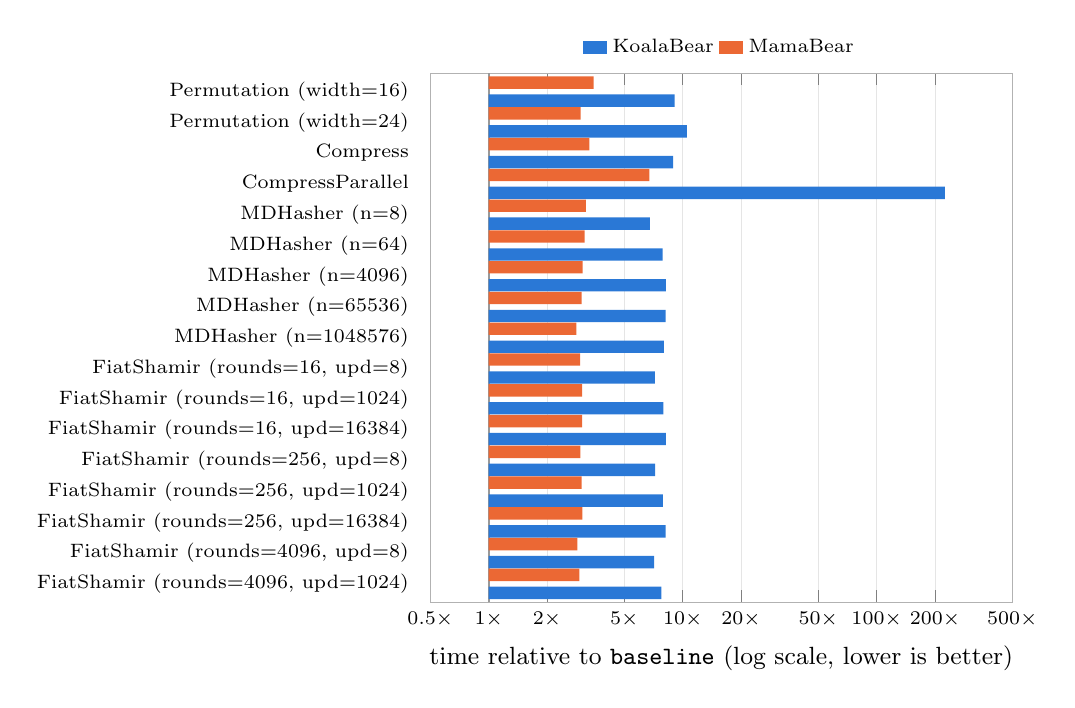
\begin{tikzpicture}
\begin{axis}[
  xbar, xmode=log, log basis x=10,
  width=0.74\linewidth, height=8.3cm,
  bar width=4.5pt, bar shift auto, enlarge y limits={abs=0.6},
  ytick={0,1,2,3,4,5,6,7,8,9,10,11,12,13,14,15,16}, yticklabels={{FiatShamir (rounds=4096, upd=1024)},{FiatShamir (rounds=4096, upd=8)},{FiatShamir (rounds=256, upd=16384)},{FiatShamir (rounds=256, upd=1024)},{FiatShamir (rounds=256, upd=8)},{FiatShamir (rounds=16, upd=16384)},{FiatShamir (rounds=16, upd=1024)},{FiatShamir (rounds=16, upd=8)},{MDHasher (n=1048576)},{MDHasher (n=65536)},{MDHasher (n=4096)},{MDHasher (n=64)},{MDHasher (n=8)},{CompressParallel},{Compress},{Permutation (width=24)},{Permutation (width=16)}},
  y tick label style={font=\scriptsize}, x tick label style={font=\scriptsize},
  xmin=0.5, xmax=500,
  xtick={0.5,1,2,5,10,20,50,100,200,500},
  xticklabels={0.5$\times$,1$\times$,2$\times$,5$\times$,10$\times$,20$\times$,50$\times$,100$\times$,200$\times$,500$\times$},
  xlabel={time relative to \texttt{baseline} (log scale, lower is better)},
  xlabel style={font=\small},
  xmajorgrids, major grid style={gray!20}, axis line style={gray!60},
  ytick style={draw=none},
  legend style={font=\scriptsize, draw=none, fill=none, at={(0.5,1.01)}, anchor=south, legend columns=-1},
  legend image code/.code={\draw[#1, draw=none] (0cm,-0.08cm) rectangle (0.3cm,0.08cm);},
  clip=false,
]
\draw[gray!80, thick] (axis cs:1,-0.6) -- (axis cs:1,16.6);
\addplot+[fill=c1, draw=none] coordinates {(9.088,16) (10.52,15) (8.923,14) (224.4,13) (6.767,12) (7.876,11) (8.182,10) (8.167,9) (8.005,8) (7.191,7) (7.95,6) (8.2,5) (7.217,4) (7.907,3) (8.156,2) (7.116,1) (7.767,0)};
\addlegendentry{KoalaBear}
\addplot+[fill=c2, draw=none] coordinates {(3.478,16) (2.979,15) (3.3,14) (6.73,13) (3.165,12) (3.122,11) (3.053,10) (3.017,9) (2.828,8) (2.961,7) (3.028,6) (3.03,5) (2.971,4) (3.016,3) (3.043,2) (2.864,1) (2.932,0)};
\addlegendentry{MamaBear}
\end{axis}
\end{tikzpicture}
\caption{Fully generic code: time relative to each field\'s \texttt{baseline} (Tables~\ref{tab:mid-kb} and \ref{tab:mid-mb}). The vertical line marks parity.}\label{fig:generic}
\end{figure}


\paragraph{How to read the tables.} Each ratio is time relative to \texttt{baseline}:
$1\times$ is the same speed, $9\times$ means nine times as long, and below $1\times$ is
faster. The allocs columns give heap allocations per operation.

\paragraph{Findings.}
\begin{itemize}
  \item KoalaBear \texttt{generic} is 6.8--10.5$\times$ slower than baseline, and MamaBear
    \texttt{generic} 2.8--3.5$\times$. Without assembly on the MamaBear side, the MamaBear
    figure is the better measure of the cost of genericity itself.
  \item \texttt{current} is on par with baseline: from 14\% faster (MDHasher, $n=8$) to
    about 2\% slower (FiatShamir). It also makes 80\% fewer allocations in MDHasher, but
    about 2.9$\times$ more in FiatShamir. The absolute numbers are small (731 vs.\ 254 at
    16 rounds), but this may deserve a look.
  \item The generic code allocates heavily: 222--340 allocations per permutation, about 28
    per absorbed element in the KoalaBear MDHasher, and up to 167 million per FiatShamir
    operation.
\end{itemize}

\paragraph{Why the generic code is slow.} Go does not compile a generic function separately
for every type. It compiles it once per ``GC shape'' (here, every \texttt{[1]uint32}-shaped
field shares the code) and passes a dictionary of the type's methods. So inside
\texttt{sBox}, \texttt{matMulM4} and the other helpers, each \texttt{PT(x).Mul},
\texttt{PT(x).Add}, \dots{} is an \emph{indirect call} through that dictionary. The compiler
cannot inline it, and it cannot see what the callee does with the pointers it receives, so
it moves the operands to the heap. That causes both the per-operation call overhead and the
hundreds of allocations per permutation.

\paragraph{Example: the internal matrix.} Every version below implements the same step of a
partial round, multiplying the state by $\mathbf{1}\mathbf{1}^T + D$: add up all elements,
then set each element to the sum plus itself times its diagonal entry. This is the fully
generic version. Each \texttt{PT(\dots)} call goes through the dictionary, and \texttt{sum}
and \texttt{tmp} are moved to the heap:
\begin{lstlisting}[language=Go,caption={Fully generic \texttt{matMulInternal} (commit \texttt{3ce6cc6e5}).},label=lst:generic]
func (h *Permutation[T, PT]) matMulInternal(input []T) {
	var sum T
	for i := range input {
		PT(&sum).Add(&sum, &input[i]) // indirect call
	}
	var tmp T
	for i := range input {
		PT(&tmp).Mul(&input[i], &h.params.InternalDiag[i]) // indirect call
		PT(&input[i]).Add(&sum, &tmp)                      // indirect call
	}
}
\end{lstlisting}
For comparison, gnark-crypto's own scalar fallback (used when there is no AVX-512) is
written for one field and one width. It never multiplies by the diagonal: the diagonal
entries are small values such as $\pm2$, $\pm\frac12$ or $2^{-8}$, so it uses doublings,
halvings and shifts instead. Since run 3, the generic code and the KoalaBear branch use
the same formula (Section~\ref{sec:replicate}); Tables~\ref{tab:mid-kb} and
\ref{tab:mid-mb} predate that change.
\begin{lstlisting}[language=Go,caption={gnark-crypto KoalaBear \texttt{matMulInternalInPlace}, width 16 (excerpt).},label=lst:gnark]
var sum fr.Element
sum.Set(&input[0])
for i := 1; i < h.params.Width; i++ {
	sum.Add(&sum, &input[i])
}
// mul by diag16: [-2, 1, 2, 1/2, 3, 4, -1/2, -3, -4, 1/2^8, ...]
var temp fr.Element
input[0].Sub(&sum, temp.Double(&input[0]))
input[1].Add(&sum, &input[1])
input[2].Add(&sum, temp.Double(&input[2]))
temp.Set(&input[3]).Halve()
input[3].Add(&sum, &temp)
// ...
input[9].Add(&sum, temp.Mul2ExpNegN(&input[9], 8))
// ...
\end{lstlisting}

\section{Results 2: branching to concrete KoalaBear code in the hot loops}\label{sec:branch}

Each hot helper of the permutation (\texttt{sBox}, \texttt{addRoundKey},
\texttt{matMulExternal} with M4, \texttt{matMulInternal}) now starts with
\texttt{if h.kb \{ \dots; return \}}. The flag \texttt{kb} is computed once in
\texttt{NewPermutation} by a type check. The KoalaBear branch reinterprets its operands as
\texttt{[]koalabear.Element} (via \texttt{unsafe}, without copying) and runs concrete loops
that the compiler can inline and keep on the stack. The check runs once per helper call;
putting it inside the per-element loops would only add work. Other fields keep the generic
code.

\begin{lstlisting}[language=Go,caption={\texttt{matMulInternal} with the hot-loop branch (\texttt{crypto/poseidon2}). The vector case belongs to Section~\ref{sec:paths}.},label=lst:branch]
// permutation.go: the generic helper branches once, on entry.
func (h *Permutation[T, PT]) matMulInternal(input []T) {
	if h.kb { // set once in NewPermutation: is T koalabear.Element?
		if h.kbPath == KoalaBearVector {
			kbMatMulInternalVec(asKB(input), asKB(h.params.InternalDiag))
			return
		}
		kbMatMulInternal(asKB(input))
		return
	}
	// ... generic code for every other field ...
}

// koalabear.go: reinterpret []T as []koalabear.Element, without copying.
func asKB[T any](s []T) []koalabear.Element {
	return unsafe.Slice((*koalabear.Element)(unsafe.Pointer(unsafe.SliceData(s))), len(s))
}

// koalabear.go: gnark-crypto's code, copied; direct calls the compiler inlines.
func kbMatMulInternal(input []koalabear.Element) {
	var sum koalabear.Element // stays on the stack
	sum.Set(&input[0])
	for i := 1; i < len(input); i++ {
		sum.Add(&sum, &input[i])
	}
	var temp koalabear.Element
	input[0].Sub(&sum, temp.Double(&input[0]))
	input[1].Add(&sum, &input[1])
	// ... as in Listing 2, for width 16 and 24 ...
}
\end{lstlisting}

\begin{table}[htbp]\centering\small
\caption{KoalaBear, the hot-loop branches before (run 2) and after (run 3) replicating gnark-crypto's internal-matrix diagonal. Each ratio is relative to the \texttt{baseline} of the same run; the baseline column shows run 3.}\label{tab:kbb}
\begin{adjustbox}{max width=\linewidth}
\begin{tabular}{lrrrrrr}
\toprule
Benchmark & baseline & branches (initial) & ratio & branches, gnark diagonal & ratio & allocs, gnark diagonal \\ \midrule
Permutation (width=16) & 570\,ns & 1.92\,\textmu s & 3.37$\times$ & 1.46\,\textmu s & 2.57$\times$ & 0 \\
Permutation (width=24) & 706\,ns & 2.63\,\textmu s & 3.73$\times$ & 2.08\,\textmu s & 2.94$\times$ & 0 \\
Compress & 585\,ns & 2.03\,\textmu s & 3.46$\times$ & 1.54\,\textmu s & 2.62$\times$ & 2 \\
CompressParallel & 4.42\,ns & 170\,ns & 38.6$\times$ & 147\,ns & 33.2$\times$ & 2 \\
MDHasher (n=64) & 4.97\,\textmu s & 16.2\,\textmu s & 3.26$\times$ & 11.8\,\textmu s & 2.38$\times$ & 17 \\
MDHasher (n=4096) & 308\,\textmu s & 1.03\,ms & 3.34$\times$ & 792\,\textmu s & 2.57$\times$ & 1\,025 \\
MDHasher (n=65536) & 4.91\,ms & 16.6\,ms & 3.37$\times$ & 12.6\,ms & 2.57$\times$ & 16\,385 \\
FiatShamir (rounds=16, upd=8) & 134\,\textmu s & 381\,\textmu s & 2.86$\times$ & 296\,\textmu s & 2.21$\times$ & 698 \\
FiatShamir (rounds=16, upd=1024) & 1.36\,ms & 4.5\,ms & 3.33$\times$ & 3.45\,ms & 2.54$\times$ & 4\,762 \\
FiatShamir (rounds=256, upd=8) & 2.11\,ms & 6.1\,ms & 2.89$\times$ & 4.8\,ms & 2.27$\times$ & 11\,013 \\
FiatShamir (rounds=256, upd=1024) & 21.7\,ms & 71.9\,ms & 3.31$\times$ & 55.4\,ms & 2.56$\times$ & 76\,046 \\
\bottomrule
\end{tabular}
\end{adjustbox}
\end{table}


\begin{figure}[htbp]\centering
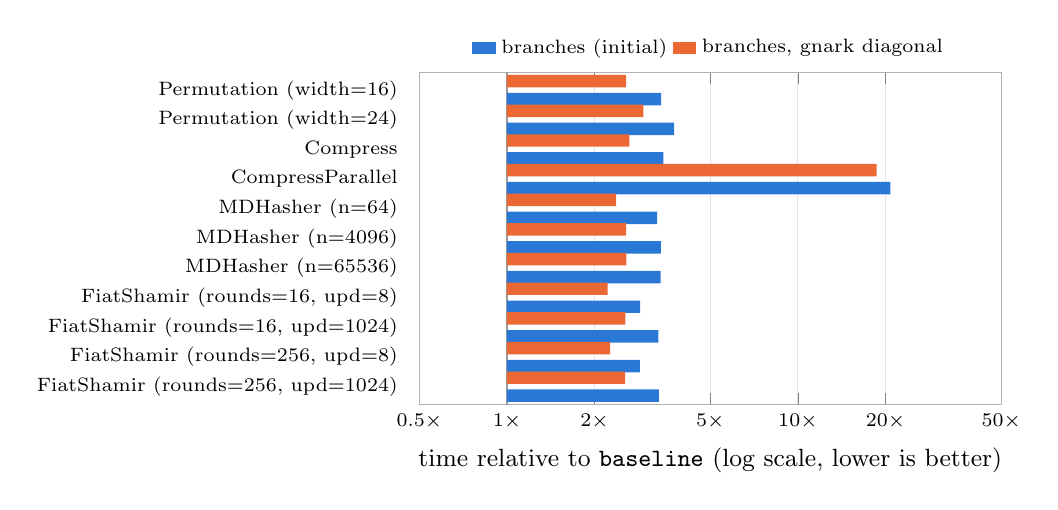
\begin{tikzpicture}
\begin{axis}[
  xbar, xmode=log, log basis x=10,
  width=0.74\linewidth, height=5.8cm,
  bar width=4.5pt, bar shift auto, enlarge y limits={abs=0.6},
  ytick={0,1,2,3,4,5,6,7,8,9,10}, yticklabels={{FiatShamir (rounds=256, upd=1024)},{FiatShamir (rounds=256, upd=8)},{FiatShamir (rounds=16, upd=1024)},{FiatShamir (rounds=16, upd=8)},{MDHasher (n=65536)},{MDHasher (n=4096)},{MDHasher (n=64)},{CompressParallel},{Compress},{Permutation (width=24)},{Permutation (width=16)}},
  y tick label style={font=\scriptsize}, x tick label style={font=\scriptsize},
  xmin=0.5, xmax=50,
  xtick={0.5,1,2,5,10,20,50,100,200,500},
  xticklabels={0.5$\times$,1$\times$,2$\times$,5$\times$,10$\times$,20$\times$,50$\times$,100$\times$,200$\times$,500$\times$},
  xlabel={time relative to \texttt{baseline} (log scale, lower is better)},
  xlabel style={font=\small},
  xmajorgrids, major grid style={gray!20}, axis line style={gray!60},
  ytick style={draw=none},
  legend style={font=\scriptsize, draw=none, fill=none, at={(0.5,1.01)}, anchor=south, legend columns=-1},
  legend image code/.code={\draw[#1, draw=none] (0cm,-0.08cm) rectangle (0.3cm,0.08cm);},
  clip=false,
]
\draw[gray!80, thick] (axis cs:1,-0.6) -- (axis cs:1,10.6);
\addplot+[fill=c1, draw=none] coordinates {(3.385,10) (3.754,9) (3.452,8) (20.77,7) (3.283,6) (3.382,5) (3.372,4) (2.87,3) (3.317,2) (2.865,1) (3.327,0)};
\addlegendentry{branches (initial)}
\addplot+[fill=c2, draw=none] coordinates {(2.57,10) (2.943,9) (2.635,8) (18.65,7) (2.371,6) (2.569,5) (2.575,4) (2.219,3) (2.554,2) (2.261,1) (2.549,0)};
\addlegendentry{branches, gnark diagonal}
\end{axis}
\end{tikzpicture}
\caption{KoalaBear hot-loop branches, time relative to \texttt{baseline}, before and after replicating gnark-crypto's internal-matrix diagonal (Table~\ref{tab:kbb}).}\label{fig:branch}
\end{figure}


\paragraph{Findings.} The permutation is now allocation-free. Its first version (run 2) was
3.4--3.7$\times$ slower than baseline. With gnark-crypto's internal-matrix formula
replicated (run 3, Section~\ref{sec:replicate}), it is 2.6--2.9$\times$ slower, and the
hashing and Fiat--Shamir benchmarks 2.2--2.6$\times$. The remaining gap is the AVX-512
assembly: one AVX-512 instruction processes 16 elements at once, which is exactly one
width-16 state, and gnark-crypto's assembly keeps the whole state in registers for all 27
rounds. Scalar Go code cannot do that. The remaining allocations (2 per compression) are
analysed in Section~\ref{sec:parallel}.

\subsection{Replicating gnark-crypto's optimisations}\label{sec:replicate}

A comparison with gnark-crypto should measure the cost of genericity, not of different
formulas. Each helper was therefore checked against gnark-crypto's scalar code for both
fields:
\begin{center}\small
\begin{adjustbox}{max width=\linewidth}
\begin{tabular}{lll}
\toprule
Step & gnark-crypto's scalar code & Our code \\ \midrule
S-box, round keys, M4, external matrix & same formulas & identical \\
Internal matrix: diagonal & doublings, \texttt{Halve}, \texttt{Mul2ExpNegN} instead of \texttt{Mul} & replicated in run 3 (generic and KoalaBear branch) \\
Internal matrix: sum, MamaBear only & raw 64-bit sum, a single reduction at the end (\texttt{sumState}) & \textbf{not replicated} \\
\bottomrule
\end{tabular}
\end{adjustbox}
\end{center}
To replicate the diagonal in the generic code, \texttt{generic.Element} gained two methods
that both fields already have, \texttt{Halve} and \texttt{Mul2ExpNegN}. The KoalaBear branch
is a line-by-line copy of gnark-crypto's function. The generic version applies the
$2^{-n}$ entries in a short loop over a table of shifts rather than unrolling them.

The effect differs by path. The KoalaBear branch became about 24\% faster
(Table~\ref{tab:kbb}). The fully generic MamaBear permutation did not: 7.69\,\textmu s in
run 3, compared with 7.27\,\textmu s in run 1, a difference within the noise of those runs.
In the generic code every field operation is an indirect call, and the formula replaces one
multiplication by two to four cheaper operations, so the number of calls, which dominates,
goes up. MamaBear's \texttt{sumState} relies on the field's internal representation and
cannot be expressed through \texttt{generic.Element}; replicating it needs a MamaBear branch
or a new interface method.

\section{Results 3: vector operations vs.\ assembly}\label{sec:paths}

Two ways to close the assembly gap were implemented side by side. The choice is made with
\texttt{SetKoalaBearPath}:
\begin{itemize}
  \item \texttt{KoalaBearScalar} (default, column ``generic + hot-loop branches''): the concrete loops of
    Section~\ref{sec:branch}.
  \item \texttt{KoalaBearVector} (\texttt{generic-vec}): the same branches, but the round
    keys, the full S-box layer and the internal matrix use gnark-crypto's batched
    \texttt{koalabear.Vector} operations (\texttt{Add}, \texttt{Mul}, \texttt{Sum}), which
    run AVX-512 loops over slices. M4 and the external matrix stay scalar because they mix
    neighbouring elements. For width 24, the last 8 elements fall back to scalar code
    because the vector operations work in blocks of 16.
  \item \texttt{KoalaBearAsm} (\texttt{generic-asm}): the branch sits at the top of
    \texttt{Permute} and hands the whole permutation to gnark-crypto's AVX-512 function.
\end{itemize}

\begin{lstlisting}[language=Go,caption={The vector path: \texttt{matMulInternal} as three batched calls (\texttt{koalabear.go}).},label=lst:vec]
func kbMatMulInternalVec(input, diag []koalabear.Element) {
	v := koalabear.Vector(input)
	sum := v.Sum()                       // AVX-512 call 1
	var buf [maxWidth]koalabear.Element  // stack scratch
	sums := koalabear.Vector(buf[:len(input)])
	for i := range sums {
		sums[i] = sum
	}
	v.Mul(v, diag)                       // AVX-512 call 2
	v.Add(v, sums)                       // AVX-512 call 3
}
\end{lstlisting}
\begin{lstlisting}[language=Go,caption={The assembly path: the branch sits at the top of \texttt{Permute}, so no helper runs at all (\texttt{permutation.go}).},label=lst:asm]
func (h *Permutation[T, PT]) Permute(input []T) error {
	// ...
	if h.kbAsm != nil { // set by SetKoalaBearPath(KoalaBearAsm)
		return h.kbAsm.Permutation(asKB(input)) // gnark-crypto: all 27 rounds in AVX-512
	}
	h.matMulExternal(input)
	// ... rounds, each calling the helpers of Listing 3 ...
}
\end{lstlisting}

\begin{table}[htbp]\centering\small
\caption{KoalaBear, the three code paths side by side (\texttt{medium} scale). \texttt{generic} is the scalar branch.}\label{tab:paths}
\begin{adjustbox}{max width=\linewidth}
\begin{tabular}{lrrrrrrrrr|r}
\toprule
Benchmark & baseline & \texttt{generic} & ratio & \texttt{generic-vec} & ratio & \texttt{generic-asm} & ratio & \texttt{current} & ratio & allocs \texttt{generic-asm} \\ \midrule
Permutation (width=16) & 570\,ns & 1.92\,\textmu s & 3.37$\times$ & 11.6\,\textmu s & 20.4$\times$ & 573\,ns & 1.01$\times$ & -- & -- & 0 \\
Permutation (width=24) & 706\,ns & 2.63\,\textmu s & 3.72$\times$ & 12.3\,\textmu s & 17.4$\times$ & 706\,ns & 1.00$\times$ & -- & -- & 0 \\
Compress & 586\,ns & 2.03\,\textmu s & 3.46$\times$ & 11.7\,\textmu s & 19.9$\times$ & 656\,ns & 1.12$\times$ & -- & -- & 2 \\
CompressParallel & 4.4\,ns & 170\,ns & 38.7$\times$ & 471\,ns & 107$\times$ & 73.2\,ns & 16.6$\times$ & -- & -- & 2 \\
MDHasher (n=64) & 4.97\,\textmu s & 16.2\,\textmu s & 3.26$\times$ & 93.4\,\textmu s & 18.8$\times$ & 5.3\,\textmu s & 1.07$\times$ & 4.88\,\textmu s & 0.98$\times$ & 17 \\
MDHasher (n=4096) & 308\,\textmu s & 1.03\,ms & 3.35$\times$ & 5.98\,ms & 19.4$\times$ & 336\,\textmu s & 1.09$\times$ & 312\,\textmu s & 1.01$\times$ & 1\,025 \\
MDHasher (n=65536) & 4.92\,ms & 16.6\,ms & 3.38$\times$ & 95.5\,ms & 19.4$\times$ & 5.34\,ms & 1.09$\times$ & 4.96\,ms & 1.01$\times$ & 16\,385 \\
FiatShamir (rounds=16, upd=8) & 133\,\textmu s & 381\,\textmu s & 2.86$\times$ & 2.08\,ms & 15.6$\times$ & 141\,\textmu s & 1.06$\times$ & 133\,\textmu s & 1.00$\times$ & 698 \\
FiatShamir (rounds=16, upd=1024) & 1.35\,ms & 4.5\,ms & 3.33$\times$ & 25.8\,ms & 19.1$\times$ & 1.5\,ms & 1.10$\times$ & 1.37\,ms & 1.01$\times$ & 4\,762 \\
FiatShamir (rounds=256, upd=8) & 2.11\,ms & 6.1\,ms & 2.89$\times$ & 33.2\,ms & 15.7$\times$ & 2.26\,ms & 1.07$\times$ & 2.13\,ms & 1.01$\times$ & 11\,013 \\
FiatShamir (rounds=256, upd=1024) & 21.7\,ms & 71.9\,ms & 3.31$\times$ & 413\,ms & 19.0$\times$ & 23.7\,ms & 1.09$\times$ & 21.9\,ms & 1.01$\times$ & 76\,043 \\
\bottomrule
\end{tabular}
\end{adjustbox}
\end{table}

\begin{figure}[htbp]\centering
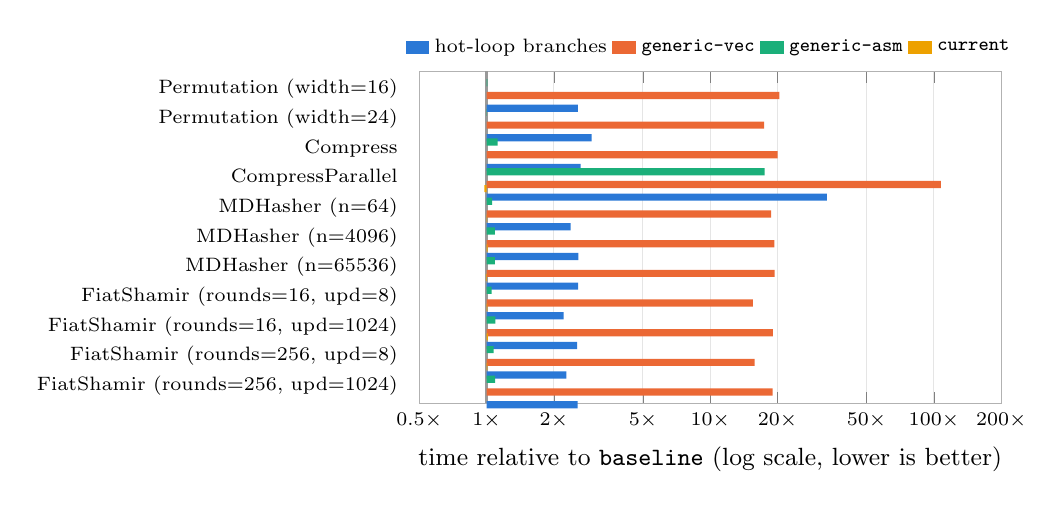
\begin{tikzpicture}
\begin{axis}[
  xbar, xmode=log, log basis x=10,
  width=0.74\linewidth, height=5.8cm,
  bar width=2.6pt, bar shift auto, enlarge y limits={abs=0.6},
  ytick={0,1,2,3,4,5,6,7,8,9,10}, yticklabels={{FiatShamir (rounds=256, upd=1024)},{FiatShamir (rounds=256, upd=8)},{FiatShamir (rounds=16, upd=1024)},{FiatShamir (rounds=16, upd=8)},{MDHasher (n=65536)},{MDHasher (n=4096)},{MDHasher (n=64)},{CompressParallel},{Compress},{Permutation (width=24)},{Permutation (width=16)}},
  y tick label style={font=\scriptsize}, x tick label style={font=\scriptsize},
  xmin=0.5, xmax=200,
  xtick={0.5,1,2,5,10,20,50,100,200,500},
  xticklabels={0.5$\times$,1$\times$,2$\times$,5$\times$,10$\times$,20$\times$,50$\times$,100$\times$,200$\times$,500$\times$},
  xlabel={time relative to \texttt{baseline} (log scale, lower is better)},
  xlabel style={font=\small},
  xmajorgrids, major grid style={gray!20}, axis line style={gray!60},
  ytick style={draw=none},
  legend style={font=\scriptsize, draw=none, fill=none, at={(0.5,1.01)}, anchor=south, legend columns=-1},
  legend image code/.code={\draw[#1, draw=none] (0cm,-0.08cm) rectangle (0.3cm,0.08cm);},
  clip=false,
]
\draw[gray!80, thick] (axis cs:1,-0.6) -- (axis cs:1,10.6);
\addplot+[fill=c1, draw=none] coordinates {(2.561,10) (2.946,9) (2.632,8) (33.26,7) (2.374,6) (2.571,5) (2.566,4) (2.209,3) (2.537,2) (2.275,1) (2.553,0)};
\addlegendentry{hot-loop branches}
\addplot+[fill=c2, draw=none] coordinates {(20.35,10) (17.42,9) (20,8) (107.5,7) (18.73,6) (19.35,5) (19.41,4) (15.52,3) (19.04,2) (15.78,1) (19.03,0)};
\addlegendentry{\texttt{generic-vec}}
\addplot+[fill=c3, draw=none] coordinates {(1.007,10) (0.9972,9) (1.12,8) (17.51,7) (1.058,6) (1.088,5) (1.088,4) (1.052,3) (1.096,2) (1.076,1) (1.092,0)};
\addlegendentry{\texttt{generic-asm}}
\addplot+[fill=c4, draw=none] coordinates {(0.9779,6) (1.006,5) (1.012,4) (0.9925,3) (1.007,2) (1.014,1) (1.009,0)};
\addlegendentry{\texttt{current}}
\end{axis}
\end{tikzpicture}
\caption{KoalaBear code paths, time relative to \texttt{baseline} (Table~\ref{tab:paths}). \texttt{current} exists only for MDHasher and FiatShamir.}\label{fig:paths}
\end{figure}


\paragraph{Findings.}
\begin{itemize}
  \item \texttt{generic-asm} matches the baseline permutation (1.00--1.01$\times$). The
    Compress, MDHasher and FiatShamir benchmarks remain 6--12\% slower than baseline. That
    overhead comes from the generic code around the permutation.
  \item \texttt{generic-vec} is about 20$\times$ slower than baseline, and about 8$\times$
    slower than the scalar branch it was meant to improve. (It still multiplies by the
    diagonal; it was not updated in run 3.) A CPU profile shows almost all the
    time inside the vector routines (75\% in the 21 partial rounds), at about 150\,ns per
    call on 16 elements. The vector routines are designed for long arrays; on a 16-element
    state the cost of each call outweighs the work. The likely cause is the penalty the CPU
    pays when switching between AVX-512 and ordinary instructions, but this has not been
    confirmed.
\end{itemize}

\paragraph{Why the two cannot be combined in one permutation.} Both paths live in the same
codebase and are compiled into the same binary; nothing conflicts. A given permutation can
use only one of them, though: the assembly function performs all 27 rounds in a single call,
so once \texttt{Permute} hands it the state, none of the per-step helpers run and there is
nowhere for a vector branch to apply. gnark-crypto does not expose the individual rounds of
its assembly. This is the underlying trade-off: branching as low as possible and matching
the baseline's speed pull in opposite directions, because the fast code exists only as one
whole-permutation block.

\section{Why CompressParallel is so slow}\label{sec:parallel}

Even with the assembly permutation, \texttt{CompressParallel} is about 17$\times$ slower than
baseline at 192 threads (Table~\ref{tab:paths}). To find out why, it was re-run at 1 to 192
threads, with the Go garbage collector (GC) on and off, and profiled at 192 threads. The
machine has 2 sockets of 48 cores, each core running 2 hardware threads, so 192 threads means
96 physical cores. The data is in \texttt{report/data/}.

\subsection{Where the allocations come from}

A memory profile attributes every allocation to two lines of the generic \texttt{Compress}
(\texttt{crypto/poseidon2/hasher.go}):
\begin{lstlisting}[language=Go,caption={Generic \texttt{Compress}. The two marked arrays are moved to the heap.},label=lst:compress]
func Compress[T any, PT generic.Element[T]](perm *Permutation[T, PT], state, block Octuplet[T]) Octuplet[T] {
	var x [CompressionWidth]T // ALLOCATES: 16 elements, 64 bytes
	copy(x[:BlockSize], state[:])
	copy(x[BlockSize:], block[:])
	if err := perm.Permute(x[:]); err != nil { // x escapes here
		panic(err)
	}
	res := block // ALLOCATES: 8 elements, 32 bytes
	for i := range res {
		PT(&res[i]).Add(&res[i], &x[BlockSize+i]) // res escapes here
	}
	return res
}
\end{lstlisting}
\begin{lstlisting}[language=Go,caption={gnark-crypto \texttt{vortex.CompressPoseidon2}: the same steps, nothing allocated.},label=lst:gnarkcompress]
func CompressPoseidon2(a, b Hash) Hash {
	res := Hash{}
	var x [16]koalabear.Element
	copy(x[:], a[:])
	copy(x[8:], b[:])
	copy(res[:], x[8:])
	if err := compressPerm.Permutation(x[:]); err != nil {
		panic(err)
	}
	for i := range res {
		res[i].Add(&res[i], &x[8+i])
	}
	return res
}
\end{lstlisting}
That is 2 allocations and 96 bytes per compression, for every generic path. These are
fixed-size local arrays and should stay on the stack, as they do in gnark-crypto's almost
identical \texttt{CompressPoseidon2}. They escape for the reason given in
Section~\ref{sec:generic}: \texttt{x} is passed to \texttt{perm.Permute} and \texttt{res}
to \texttt{PT(\&res[i]).Add}, both indirect calls the compiler cannot see through, so it
assumes the pointers may be kept and moves both arrays to the heap.

\subsection{Scaling with the number of threads}

\begin{table}[htbp]\centering\small
\caption{KoalaBear CompressParallel, nanoseconds per compression (lower is better) by number of threads (\texttt{-cpu}), with the garbage collector on (default) and off (\texttt{GOGC=off}). Ratios are relative to \texttt{baseline} at the same thread count. \texttt{baseline} allocates nothing, so the GC setting does not affect it.}\label{tab:parallel}
\begin{adjustbox}{max width=\linewidth}
\begin{tabular}{rr|rrrr|rrrr}
\toprule
 & & \multicolumn{4}{c|}{\texttt{generic-asm}} & \multicolumn{4}{c}{generic + hot-loop branches} \\
Threads & baseline & GC on & ratio & GC off & ratio & GC on & ratio & GC off & ratio \\ \midrule
1 & 584 & 652 & 1.1$\times$ & 647 & 1.1$\times$ & 1560 & 2.7$\times$ & 1620 & 2.8$\times$ \\
2 & 292 & 335 & 1.1$\times$ & 325 & 1.1$\times$ & 785 & 2.7$\times$ & 828 & 2.8$\times$ \\
4 & 146 & 173 & 1.2$\times$ & 158 & 1.1$\times$ & 395 & 2.7$\times$ & 397 & 2.7$\times$ \\
8 & 73.3 & 106 & 1.5$\times$ & 80.8 & 1.1$\times$ & 212 & 2.9$\times$ & 193 & 2.6$\times$ \\
16 & 38.8 & 82.3 & 2.1$\times$ & 42.1 & 1.1$\times$ & 144 & 3.7$\times$ & 104 & 2.7$\times$ \\
32 & 21.7 & 80.4 & 3.7$\times$ & 24.0 & 1.1$\times$ & 142 & 6.5$\times$ & 58.2 & 2.7$\times$ \\
48 & 16.0 & 90.0 & 5.6$\times$ & 18.1 & 1.1$\times$ & 170 & 11$\times$ & 54.3 & 3.4$\times$ \\
64 & 12.8 & 103 & 8.1$\times$ & 14.6 & 1.1$\times$ & 214 & 17$\times$ & 51.2 & 4.0$\times$ \\
\bottomrule
\end{tabular}
\end{adjustbox}
\end{table}

\begin{figure}[htbp]\centering
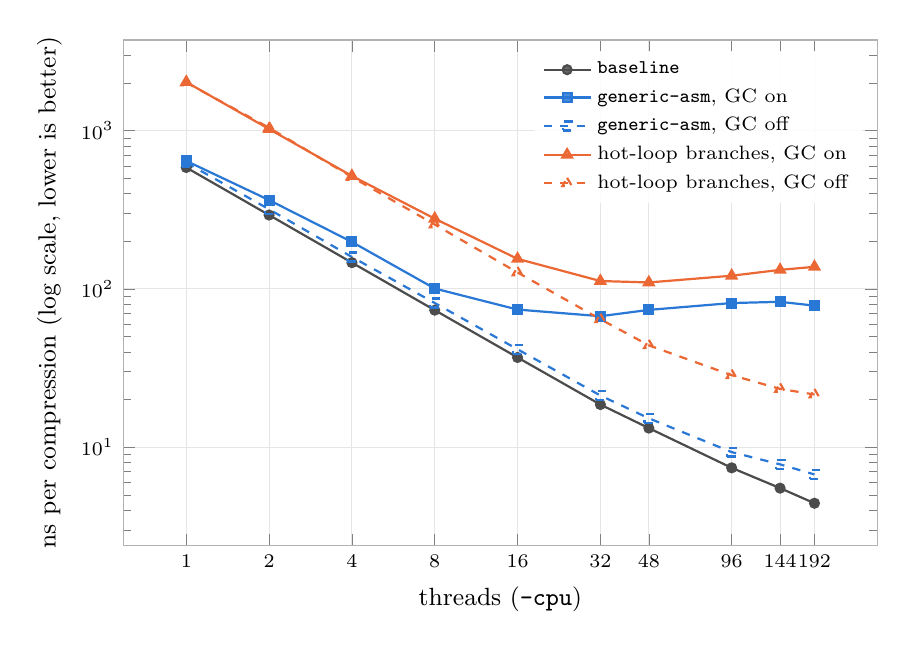
\begin{tikzpicture}
\begin{axis}[
  xmode=log, ymode=log, log basis x=2,
  width=0.92\linewidth, height=8cm,
  xtick={1,2,4,8,16,32,48,96,144,192}, xticklabels={1,2,4,8,16,32,48,96,144,192},
  xlabel={threads (\texttt{-cpu})}, ylabel={ns per compression (log scale, lower is better)},
  label style={font=\small}, tick label style={font=\scriptsize},
  grid=major, major grid style={gray!20}, axis line style={gray!60},
  legend style={font=\scriptsize, draw=none, fill=white, fill opacity=0.85, text opacity=1, at={(0.98,0.98)}, anchor=north east},
  legend cell align=left,
]
\addplot[black!70, thick, mark=*, mark size=1.6pt] coordinates {(1,585.1) (2,293.1) (4,146.6) (8,73.44) (16,36.89) (32,18.6) (48,13.2) (96,7.405) (144,5.511) (192,4.424)};
\addlegendentry{\texttt{baseline}}
\addplot[c1, thick, mark=square*, mark size=1.6pt] coordinates {(1,644.1) (2,364.4) (4,198.1) (8,100.6) (16,74.06) (32,67.25) (48,73.73) (96,81.44) (144,82.9) (192,78.44)};
\addlegendentry{\texttt{generic-asm}, GC on}
\addplot[c1, thick, dashed, mark=square, mark size=1.6pt] coordinates {(1,627.6) (2,318.7) (4,159.2) (8,81.47) (16,41.56) (32,21.21) (48,15.23) (96,9.309) (144,7.791) (192,6.726)};
\addlegendentry{\texttt{generic-asm}, GC off}
\addplot[c2, thick, mark=triangle*, mark size=2pt] coordinates {(1,2028) (2,1024) (4,517.6) (8,278) (16,154.9) (32,112.2) (48,109.9) (96,121.2) (144,132) (192,138)};
\addlegendentry{hot-loop branches, GC on}
\addplot[c2, thick, dashed, mark=triangle, mark size=2pt] coordinates {(1,2014) (2,1044) (4,509.1) (8,255.4) (16,127) (32,64.36) (48,44) (96,28.51) (144,23.36) (192,21.52)};
\addlegendentry{hot-loop branches, GC off}
\end{axis}
\end{tikzpicture}
\caption{KoalaBear CompressParallel scaling (Table~\ref{tab:parallel}). Solid: garbage collector on (default); dashed: off. Colour follows the implementation.}\label{fig:parallel}
\end{figure}


Table~\ref{tab:parallel} shows the key result:
\begin{itemize}
  \item \textbf{With the GC on}, \texttt{generic-asm} keeps up with baseline only up to
    about 8 threads. It reaches its best time at 32 threads (67\,ns) and then gets
    \emph{slower} as threads are added (76--86\,ns from 48 threads on). Baseline keeps
    improving to 4.6\,ns, so the ratio grows from 1.1$\times$ to 16$\times$. The branched
    scalar path behaves the same way (best 96\,ns at 32 threads, 27$\times$ at 192).
  \item \textbf{With the GC off}, \texttt{generic-asm} scales almost as well as baseline:
    1.1--1.5$\times$ at every thread count, 7.1\,ns at 192 threads. The scalar path stays at
    2.6--3.9$\times$, close to its single-threaded ratio.
\end{itemize}
So the parallel slowdown is caused almost entirely by \textbf{garbage collection}, not by
allocation itself and not by the permutation. Allocating without collecting costs
10--50\% (the remaining gap with the GC off).

\subsection{Why garbage collection hurts this much}

A CPU profile of \texttt{generic-asm} at 192 threads (2\,s run, taken before run 3; the
assembly path does not use the code changed in run 3) shows:
\begin{itemize}
  \item \textbf{289 GC cycles} during the run with the GC on, about one every 20\,ms. With
    the GC off there were 13, all forced by the test framework between runs.
  \item \textbf{Less than half the CPU in use.} With the GC on, the profile recorded
    95\,CPU-seconds over the run; with it off, 203\,CPU-seconds over the same duration, and
    4.1$\times$ more compressions completed. The difference is time threads spent stopped or
    waiting, which a CPU profile does not show directly.
  \item Of the CPU time that was used with the GC on, about 7\% went to background
    marking (\texttt{gcBgMarkWorker}), 4\% to mark assists (\texttt{gcAssistAlloc}),
    11\% to allocation (\texttt{mallocgc}), and the rest of the runtime share to locking,
    spinning and scheduling (\texttt{lfstack.pop}, \texttt{futex}, \texttt{procyield},
    \texttt{schedule}).
\end{itemize}
The mechanism:
\begin{enumerate}
  \item \textbf{The live heap is tiny} (about 4\,MB). With the default \texttt{GOGC=100}, a
    GC cycle starts whenever the heap doubles, here every \textasciitilde5\,MB allocated.
  \item \textbf{192 threads allocate fast}: 96 bytes per compression at about 15 million
    compressions per second is about 1.5\,GB/s, so a new cycle starts every few
    milliseconds.
  \item \textbf{Each cycle costs every thread.} A cycle stops the world twice, which means
    waiting for all 192 threads to reach a safe point. During marking, a quarter of the
    threads are taken for background mark workers, and threads that allocate are made to
    help with marking (assists). Synchronising all of this across 192 threads and two
    sockets dominates.
  \item \textbf{More threads make it worse.} Adding threads raises the allocation rate, so
    cycles come more often and each one has more threads to coordinate. Past about 32
    threads, extra threads add more GC cost than useful work.
\end{enumerate}

\subsection{Caveats}
\begin{itemize}
  \item The benchmark is close to a worst case. In the prover the live heap is much larger,
    so with \texttt{GOGC=100} cycles are much rarer (but each one marks more). The real
    impact depends on the prover's heap and its other allocations. The fix is the same
    either way: make \texttt{Compress} allocation-free.
  \item Above 96 threads the extra threads are hyperthreads sharing a core. Even baseline
    gains only 1.7$\times$ from 96 to 192 threads.
  \item The profiled runs used a 2\,s benchtime and are slower than the table (profiling a
    192-thread process has overhead). The comparison between GC on and off is between runs
    with identical settings.
  \item The same two allocations account for the 16\,385 allocations of MDHasher at
    $n=65\,536$, so they also matter single-threaded at a smaller scale (6--12\%).
\end{itemize}

\section{Recommendations}

\begin{enumerate}
  \item \textbf{Make \texttt{KoalaBearAsm} the default} when the CPU supports AVX-512 and the
    parameters are 6 full and 21 partial rounds; otherwise fall back to the scalar branch.
  \item \textbf{Remove the two allocations in \texttt{Compress}} by applying the same
    KoalaBear branch there: reinterpret \texttt{x} and \texttt{res} as KoalaBear arrays and
    do the feed-forward with direct calls. A per-permutation scratch buffer would not work,
    as it would break concurrent use.
  \item \textbf{Drop \texttt{KoalaBearVector}}, or keep it only as a recorded negative
    result.
  \item \textbf{For MamaBear} (about 3.5$\times$, with no assembly available), the overhead is
    purely the generic code. Closing it means concrete branches like KoalaBear's, which would
    also be the place to replicate gnark-crypto's \texttt{sumState}
    (Section~\ref{sec:replicate}).
  \item Look into the higher allocation count of \texttt{current} in FiatShamir (about
    2.9$\times$ baseline).
\end{enumerate}

\appendix
\section{Reproducing}

From \texttt{prover-ray/}, with \texttt{benchstat} installed
(\texttt{go install golang.org/x/perf/cmd/benchstat@latest}):
\begin{lstlisting}
# all fields, medium scale (a few minutes)
scripts/bench-generic-poseidon.sh medium <outdir>

# KoalaBear only, as in run 3 (about 80 s)
go test ./crypto/genericbench/ -run TestAgreement
GENERIC_BENCH_SCALE=medium go test ./crypto/genericbench/ -run '^$' \
  -bench '/field=koalabear/' -benchmem -count 6 -benchtime 200ms > raw.txt
benchstat -col /impl raw.txt
\end{lstlisting}

\end{document}
